\chapter{Proposed System Architecture}
\section{System Overview}
The proposed system introduces a RAG--based architecture to address the scalability and latency limitations observed in the existing Meadow9+ chatbot, which directly supplies entire meeting transcripts to a self-hosted LLM. The redesigned architecture decomposes the end-to-end pipeline into modular components for transcript processing, retrieval, and generation, enabling efficient querying over long-duration and noisy speech-to-text data.\cite{gao2024retrieval}

To minimise disruption to the existing Meadow9+ infrastructure, the new retrieval system is deployed as a separate retrieval server that interacts with the current Meadow9+ backend server. This separation reduces the extent of modifications required on the production backend, while enabling the possibility of controlled A/B testing in production to compare the performance of the existing chatbot approach against the new retrieval pipeline proposed in this project.

In the redesigned workflow, when a user submits a new recording and a corresponding transcription is generated, the transcript continues to be stored in the existing database as per the current implementation. In addition, the same transcript is forwarded to the retrieval server, where it is parsed, embedded, and indexed for retrieval, as illustrated in Figure \ref{fig:system-integration}. This ensures that the proposed retrieval system can be integrated incrementally alongside the existing system, while maintaining backward compatibility and enabling direct evaluation under real usage conditions.

\begin{figure}[H]
  \centering
  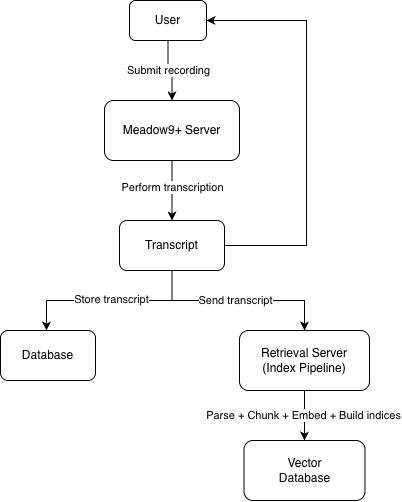
\includegraphics[width=0.7\textwidth]{figures/image4.png}
  \caption{System integration: transcript indexing pipeline}
  \label{fig:system-integration}
\end{figure} 

At a high level, the retrieval system operates in two distinct phases: an indexing phase and an query phase.

During indexing, raw speech-to-text transcripts in SubRip (SRT) format are parsed, segmented, embedded, and stored in a persistent vector database alongside auxiliary keyword-based indices. Figure \ref{fig:indexing-pipeline} shows the complete indexing pipeline, including processing, chunking, and embedding stages.

\begin{figure}[H]
  \centering
  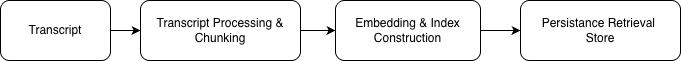
\includegraphics[width=1.0\textwidth]{figures/image5.png}
  \caption{Indexing pipeline: processing, chunking, and embedding stages}
  \label{fig:indexing-pipeline}
\end{figure} 

During querying, user questions are transformed into embeddings, used to retrieve a small set of relevant transcript segments, and supplied to the LLM as contextual grounding for response generation. This query workflow is depicted in Figure \ref{fig:query-workflow}, with the complete RAG pipeline architecture shown in Figure \ref{fig:rag-pipeline}.\cite{gao2024retrieval}

\begin{figure}[H]
  \centering
  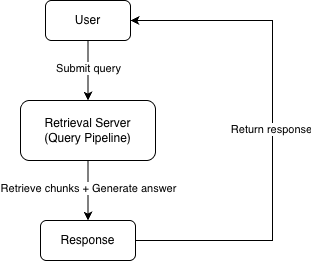
\includegraphics[width=0.54\textwidth]{figures/image6.png}
  \caption{Query phase: retrieval and response generation}
  \label{fig:query-workflow}
\end{figure} 

\begin{figure}[H]
  \centering
  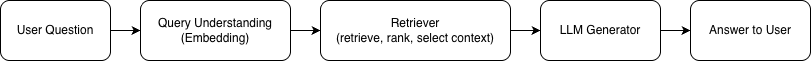
\includegraphics[width=1.0\textwidth]{figures/image7.png}
  \caption{RAG pipeline: query-to-response architecture}
  \label{fig:rag-pipeline}
\end{figure}

\section{Retriever System Architecture}

\subsection{Initial Retrieval}
At query time, the user question is first embedded using the same embedding model as the indexed chunks. As shown in Figure \ref{fig:hybrid-retrieval}, four retrieval strategies are then executed in parallel: semantic similarity search over the vector database, keyword-based retrieval using BM25, phonetic search, and fuzzy matching.\cite{robertson2009bm25,black2021doublemetaphone,levenshtein1965} Each retriever returns a ranked list of candidate transcript chunks.

\begin{figure}[H]
  \centering
  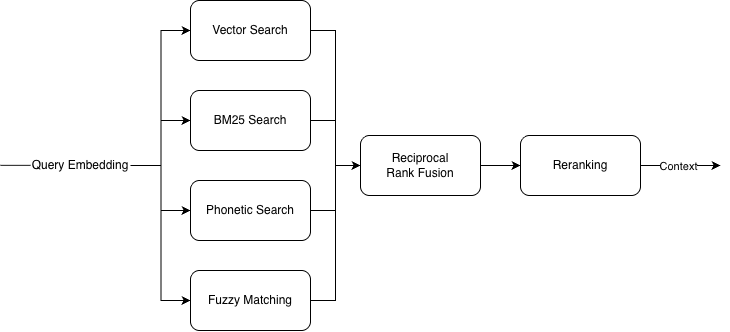
\includegraphics[width=1.0\textwidth]{figures/image8.png}
  \caption{Hybrid retrieval: multi-signal fusion and reranking}
  \label{fig:hybrid-retrieval}
\end{figure}

This hybrid design is motivated by the nature of speech-to-text transcripts, which frequently contain recognition errors, disfluencies, and domain-specific terminology.\cite{metzger2024measuring} Semantic retrieval captures paraphrased or conceptually related content, while BM25 remains effective for exact keyword matches and rare terms.\cite{robertson2009bm25} Phonetic search improves recall when proper nouns or technical phrases are mis-transcribed into similar-sounding variants, and fuzzy matching further mitigates minor spelling inconsistencies and token-level noise.\cite{black2021doublemetaphone,levenshtein1965} Together, these complementary signals increase retrieval robustness under noisy transcription conditions.

\subsection{Rank Fusion and Reranking}
The outputs of the semantic, lexical, and phonetic retrieval components are combined using Reciprocal Rank Fusion (RRF), which normalises rankings across heterogeneous retrieval functions and prioritises candidates that are consistently ranked highly across multiple retrievers.\cite{cormack2009reciprocal} RRF was selected due to its simplicity, robustness, and strong empirical performance in information retrieval systems.

A cross-encoder reranker is then applied to the fused candidate set.\cite{nogueira2019passage} The reranker jointly encodes the query and each candidate chunk to compute fine-grained relevance scores, improving precision at the top ranks. To ensure system robustness, the architecture is designed to degrade gracefully: if the reranker service is unavailable, the system falls back to the fused ranking without interrupting query processing.

\section{Evaluation System Architecture}
\subsection{Dataset Preparation}
To enable systematic evaluation, a dedicated pipeline generates question--answer pairs from transcript data using an external LLM, as illustrated in Figure \ref{fig:dataset-generation}. Transcript segments are grouped into medium-sized context windows, from which multiple self-contained questions are generated. Each question is annotated with the corresponding timestamp range, forming a temporally grounded ground truth dataset.

\begin{figure}[H]
  \centering
  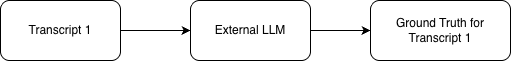
\includegraphics[width=0.7\textwidth]{figures/image9.png}
  \caption{Dataset generation: QA pair creation from transcripts}
  \label{fig:dataset-generation}
\end{figure}

\subsection{Automated Evaluation Pipeline}
Figure \ref{fig:evaluation-pipeline} shows the evaluation architecture, which mirrors the query pipeline (RAG system) but operates in batch mode. For each question, the system performs retrieval, generates an answer, and computes retrieval and generation metrics. Retrieval effectiveness is assessed using hit rate and mean reciprocal rank (MRR) based on timestamp overlap,\cite{wikipedia2024mrr} while generation quality is measured using token-level F1 score and an LLM-based semantic judge.\cite{vanrijsbergen1979ir}

\begin{figure}[H]
  \centering
  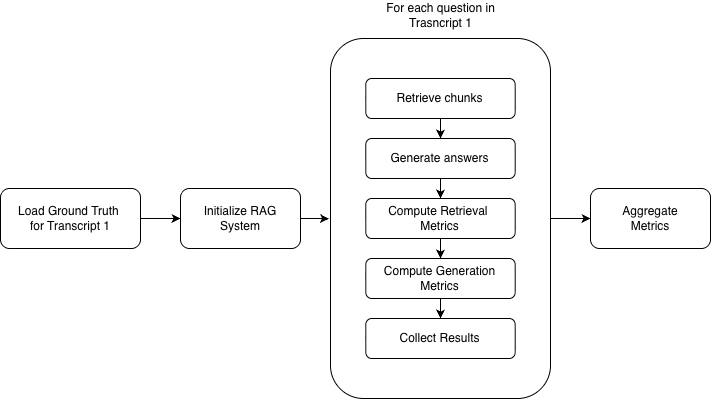
\includegraphics[width=1.0\textwidth]{figures/image10.png}
  \caption{Evaluation pipeline: retrieval and generation metrics}
  \label{fig:evaluation-pipeline}
\end{figure}

Crucially, retrieval metrics are computed before generation, ensuring that retrieval and generation errors can be diagnosed independently.

\subsection{Speed Benchmarking Setup}
A separate benchmarking pipeline compares the RAG-based system against a pure LLM baseline that consumes truncated full transcripts, as shown in Figure \ref{fig:speed-benchmark}. Queries are executed in an interleaved manner to mitigate caching effects, and component-level timings are recorded to isolate retrieval and generation costs. This design enables fair and reproducible latency comparisons across different transcript lengths.

\begin{figure}[H]
  \centering
  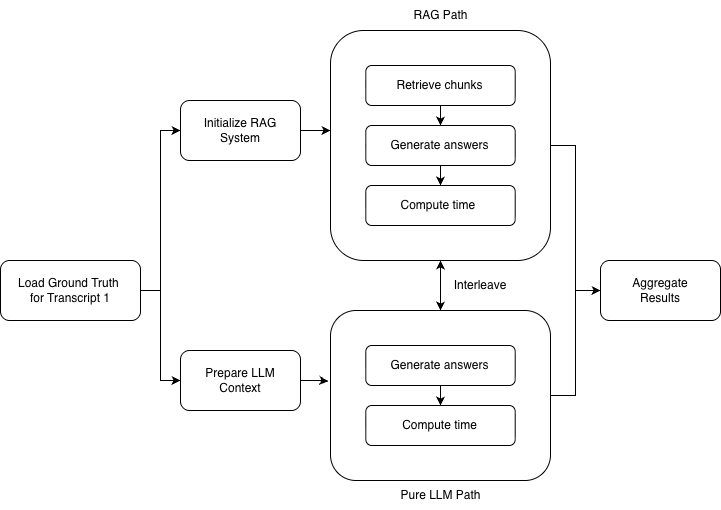
\includegraphics[width=1.0\textwidth]{figures/image11.png}
  \caption{Benchmarking: RAG vs. pure LLM comparison}
  \label{fig:speed-benchmark}
\end{figure}
